\documentclass[border=10pt]{standalone}

\usepackage{tikz}
\usetikzlibrary{arrows,shapes,positioning,shadows,trees}

\renewcommand\familydefault{\sfdefault}

\tikzset{
  basic/.style  = {draw, text width=4cm, drop shadow, font=\sffamily, rectangle},
  root/.style   = {basic, rounded corners=2pt, thin, align=center,
                   fill=gray!20},
  level 2/.style = {basic, rounded corners=6pt, thin,align=center, fill=gray!5,
                   text width=8em},
  level 3/.style = {basic, thin, align=left, fill=gray!0, text width=5em}
}

\begin{document}
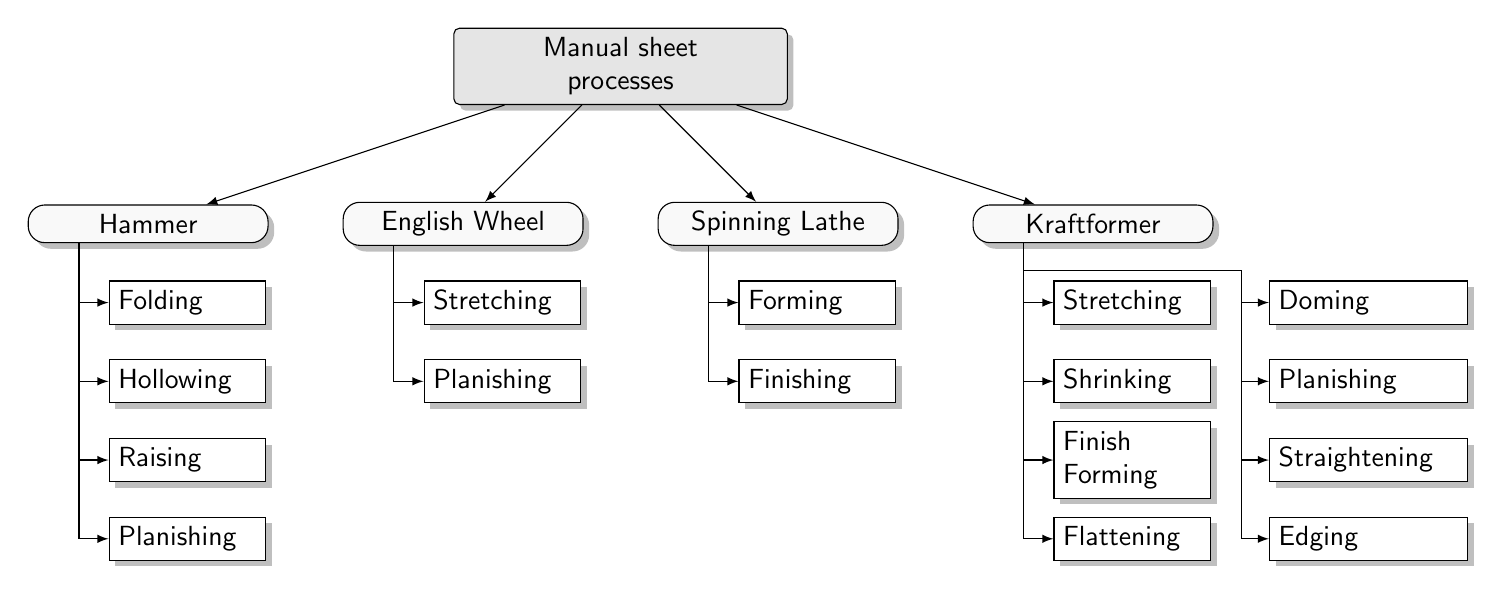
\begin{tikzpicture}[
  level 1/.style={sibling distance=40mm},
  edge from parent/.style={->,draw},
  >=latex]

%\draw[help lines, color=gray!30, dashed] (0,0) grid (20,12);

\node[root] at (10,10) (Start) {Manual sheet \\ processes};

\foreach \x [count=\xi] in {Hammer, English Wheel, Spinning Lathe, Kraftformer}{
    \pgfmathsetmacro\result{\xi * 4}
    \node[level 2] at (\result,8) (\x) {\x};
    \draw[->] (Start) -- (\x);
    }

\foreach \x [count=\xi] in {Folding, Hollowing, Raising, Planishing}{
    \pgfmathsetmacro\result{\xi * -1 +8}
    \node[level 3] at (4.5,\result) (\x) {\x};
    \draw[->] ([xshift=-2.5em)]Hammer.south) |- (\x);
    }


\foreach \x [count=\xi] in {Stretching, Planishing}{
    \pgfmathsetmacro\result{\xi * -1 +8}
    \node[level 3] at (8.5,\result) (\x) {\x};
    \draw[->] ([xshift=-2.5em)]English Wheel.south) |- (\x);
    }
    
\foreach \x [count=\xi] in {Forming, Finishing}{
    \pgfmathsetmacro\result{\xi * -1 +8}
    \node[level 3] at (12.5,\result) (\x) {\x};
    \draw[->] ([xshift=-2.5em)]Spinning Lathe.south) |- (\x);
    }
    
\foreach \x [count=\xi] in {Stretching,Shrinking,Finish Forming, Flattening}{
    \pgfmathsetmacro\result{\xi * -1 +8}
    \node[level 3] at (16.5,\result) (\x) {\x};
    \draw[->] ([xshift=-2.5em)]Kraftformer.south) |- (\x);
    }
    
\foreach \x [count=\xi] in {Doming,Planishing,Straightening,Edging}{
    \pgfmathsetmacro\result{\xi * -1 +8}
    \node[level 3,text width=6.5em] at (19.5,\result) (\x) {\x};
    \draw[->] ([xshift=-2.5em,yshift=-1em)]Kraftformer.south) -| ([xshift=-1em]\x.west) |- (\x);
    }


\end{tikzpicture}
\end{document}